\documentclass[12pt,titlepage]{article}
\usepackage[margin=1.25in]{geometry}
\usepackage{graphicx,amsmath,blindtext,minted}

%% Variables definition
\newcommand{\vSubject}{Basic Programming Practicum}
\newcommand{\vSubtitle}{Jobsheet 8 Array 1}
\newcommand{\vName}{Dicha Zelianivan Arkana}
\newcommand{\vNIM}{2241720002}
\newcommand{\vClass}{1i}
\newcommand{\vDepartment}{Information Technology}
\newcommand{\vStudyProgram}{D4 Informatics Engineering}

%% [START] Tikz related stuff
\usepackage{tikz}
\usetikzlibrary{svg.path,calc,shapes.geometric,shapes.misc}
\tikzstyle{terminator} = [rectangle, draw, text centered, rounded corners = 1em, minimum height=2em]
\tikzstyle{preparation} = [chamfered rectangle, chamfered rectangle sep=0.75em, draw, text centered, minimum height = 2em]
\tikzstyle{process} = [rectangle, draw, text centered, minimum height=2em]
\tikzstyle{decision} = [diamond, aspect=2, draw, text centered, minimum height=2em]
\tikzstyle{data}=[trapezium, draw, text centered, trapezium left angle=60, trapezium right angle=120, minimum height=2em]
\tikzstyle{connector} = [line width=0.25mm,->]
%% [END] Tikz related stuff

%% [START] Fancy header related stuff
\usepackage{fancyhdr}
\pagestyle{fancy}
\setlength{\headheight}{15pt} % compensate fancyhdr style
\fancyhead{}
\fancyfoot{}
\fancyfoot[L]{\thepage}
\fancyfoot[R]{\textit{\vSubject - \vSubtitle}}
\renewcommand{\footrulewidth}{0.4pt}% default is 0pt, overline for footer
%% [END] Fancy header related stuff

%% [START] Custom tabular command related stuff
\usepackage{tabularx}
\newcommand{\details}[2]{
    #1 & #2  \\
}
%% [END] Custom tabular command related stuff

%% [START] Figure related stuff
\newcommand{\image}[3][1]{
    \begin{figure}[h]
        \centering
        \includegraphics[#1]{#2}
        \caption{#3}
        \label{#3}
    \end{figure}
}
%% [END] Figure related stuff

\begin{document}
\begin{titlepage}
    \centering
    \vfill
    {\bfseries\LARGE
        \vSubject\\
        \vskip0.25cm
        \vSubtitle
    }
    \vfill
    
\includegraphics[width=6cm]{images/polinema-logo.png}
    \vfill
    {
        \textbf{Name}\\
        \vName\\
        \vskip0.5cm
        \textbf{NIM}\\
        \vNIM\\
        \vskip0.5cm
        \textbf{Class}\\
        \vClass\\
        \vskip0.5cm
        \textbf{Department}\\
        \vDepartment\\
        \vskip0.5cm
        \textbf{Study Program}\\
        \vStudyProgram
    }
\end{titlepage}

\section{Laboratory}
\subsection{Experiment 1: Fill in Array Element}
\begin{enumerate}
    \item Create a new project
    \item Create a new class, name it \textbf{myArray}
    \item Write the basic structure of the Java programming language which contains the \texttt{main()} function
    \item {
        Create an array of integer type named \texttt{num} with a capacity of 4 elements

        \begin{minted}[autogobble]{java}
            int[] num = new int[4];
        \end{minted}
    }
    \item {
        Fill each element of the array with numbers 5, 12, 7, 20

        \begin{minted}[autogobble]{java}
            num[0] = 5;
            num[1] = 12;
            num[2] = 7;
            num[3] = 20;
        \end{minted}
    }
    \item {
        Display all contents of the elements to the screen

        \begin{minted}[autogobble]{java}
            System.out.println(num[0]);
            System.out.println(num[1]);
            System.out.println(num[2]);
            System.out.println(num[3]);
        \end{minted}
    }
    \pagebreak
    \item {
        Compile and run the program. Match the result of the running programs that you have created according to the following display

        \begin{minted}[autogobble]{bash}
            5
            12
            7
            20
        \end{minted}

        \begin{figure}[h]
            \centering
            \fbox{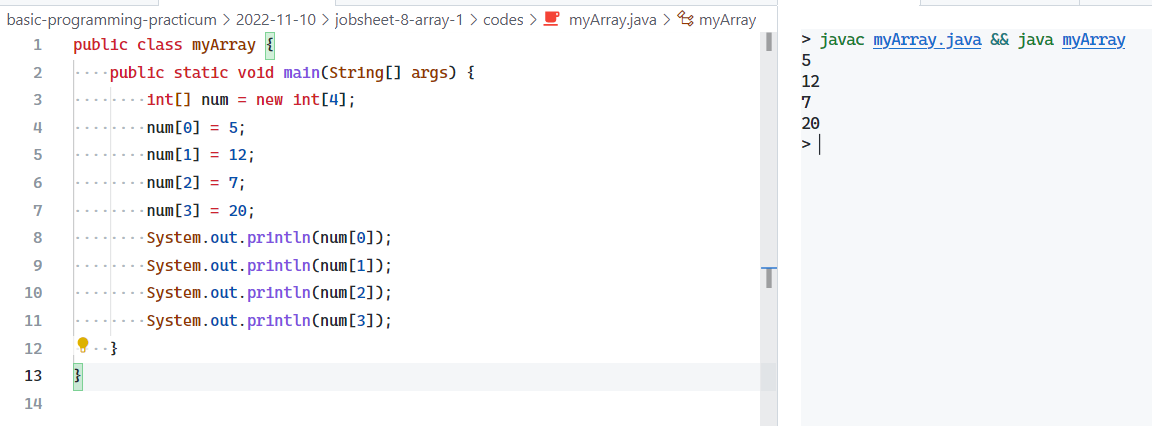
\includegraphics[width=.9\textwidth]{./images/myArray.png}}
            \caption{Experiment 1 code and output}
        \end{figure}
    }
\end{enumerate}
\subsubsection*{Questions}
\begin{enumerate}
    \item {
        In Experiment 1, what are the largest and smaller array indexes?

        The smallest array index is \texttt{0} and the largest is \texttt{3}
    }
    \item {
        If the contents of each element of the array \texttt{num} are changed with numbers
        \texttt{5.0, 12867, 7.5, 2000000}. What happens? How can it be like that?

        The fractions will be truncated because we used the \texttt{int} type for our array which couldn't store fractions.
        Every elements in an array must have the same data type.
    }
    \item {
        Change the statement in step 6 to be like this

        \begin{minted}[autogobble]{java}
            for (int i = 0; i < 4; i++) {
                System.out.println(num[i]);
            }
        \end{minted}

        What is the result? How can it be like that?

        The result is still the same because we used the looping construct instead of copying and pasting the lines manually.
        They both do the same thing, which is doing \texttt{System.out.println()} 4 times.
    }
\end{enumerate}
\subsection{Experiment 2: Requesting User Input to Fill in an Array Element}
\begin{enumerate}
    \item Create a new class, name it \textbf{arrayInputLoop}
    \item Write the basic structure of the Java programming language which contains the \texttt{main()} function
    \item Add the Scanner library
    \item Make a \textbf{Scanner} declaration with the name \texttt{sc}
    \item {
        Create an array of integer type with the name \texttt{finalSCore}, with a capacity of 6 elements

        \begin{minted}[autogobble]{java}
            int[] finalScore = new int[6];
        \end{minted}
    }
    \item {
        Using a loop, create an input to fill in the \texttt{finalSCore} array element
        
        \begin{minted}[autogobble]{java}
            for (int i = 0; i < 6; i++) {
                System.out.print("Enter the final score " + i + ": ");
                finalScore[i] = sc.nextInt();
            }
        \end{minted}
    }
    \item {
        Using a loop, display all the contents of the elements from the \texttt{finalScore} array

        \begin{minted}[autogobble]{java}
            for (int i = 0; i < 6; i++) {
                System.out.println("Final score " + i + " is " + finalScore[i]);
            }
        \end{minted}
    }
    \pagebreak
    \item {
        Compile and run the program. Match the results of the running programs that you have created according to the following display

        \begin{minted}[autogobble]{bash}
            Enter the final score 0: 88
            Enter the final score 1: 90
            Enter the final score 2: 74
            Enter the final score 3: 83
            Enter the final score 4: 92
            Enter the final score 5: 77
            Final score 0 is 88
            Final score 1 is 90
            Final score 2 is 74
            Final score 3 is 83
            Final score 4 is 92
            Final score 5 is 77
        \end{minted}

        \begin{figure}[h]
            \centering
            \fbox{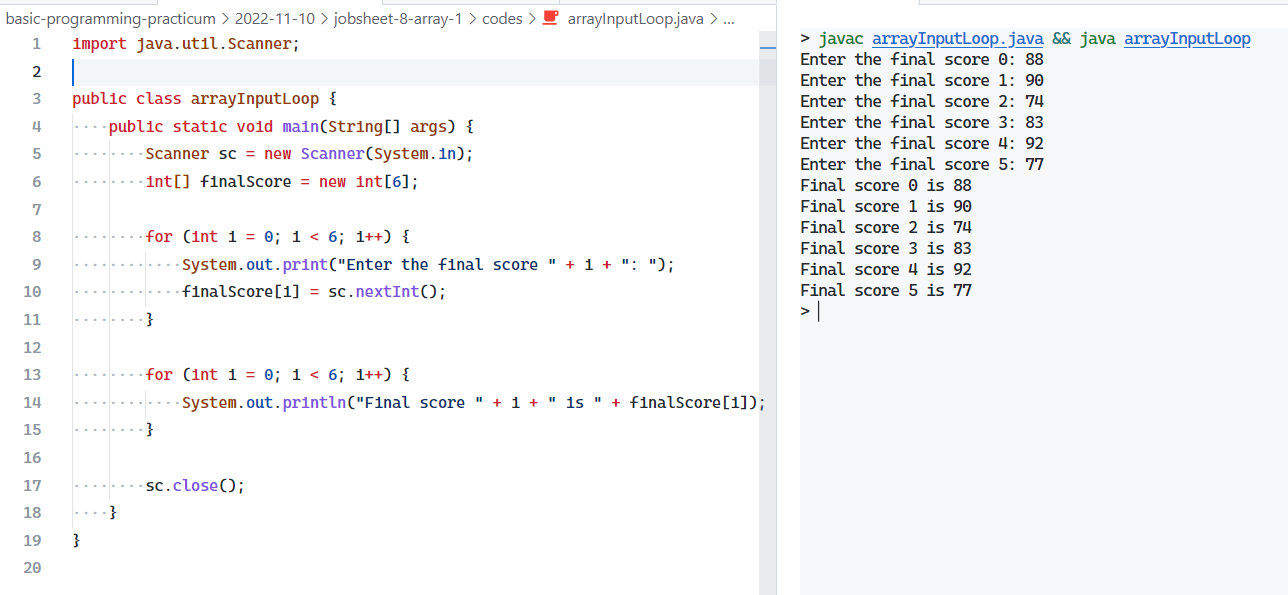
\includegraphics[width=.9\textwidth]{./images/arrayInputLoop.png}}
            \caption{Experiment 2 code and output}
        \end{figure}
    }
\end{enumerate}
\subsubsection*{Questions!}
\begin{enumerate}
    \item {
        Change the statement in step 6 to be like this

        \begin{minted}[autogobble]{java}
            for (int i = 0; i < finalScore.length; i++) {
                System.out.println("Enter the final score " + i + ": ");
                finalScore[i] = sc.nextInt();
            }
        \end{minted}

        Run the program. Have there been any changes? How can it be like that?

        There is no changes. The reason is because instead of using a hardcoded value \texttt{6}, we now use the property \texttt{.length} from the \texttt{finalScore} array.
    }
    \item {
        What is the use of \texttt{finalScore.length}?

        It is used to get the length of the \texttt{finalScore} array.
    }
    \item {
        Change the statement in step 7 to be like this, so that the program only displays the grades of students who passed

        \begin{minted}[autogobble]{java}
            for (int i = 0; i < finalScore.length; i++) {
                if (finalScore[i] > 70) {
                    System.out.println("Final score " + i + " is " + finalScore[i]);
                }
            }
        \end{minted}

        Run the program and describe the flow of the program!

        \textbf{Program Flow}
        \begin{itemize}
            \item It initialises the \texttt{for} loop
            \item It checks if the current score is higher than 70
            \item If the current score is higher than 70, then print the score
        \end{itemize}

        \begin{figure}[h]
            \centering
            \fbox{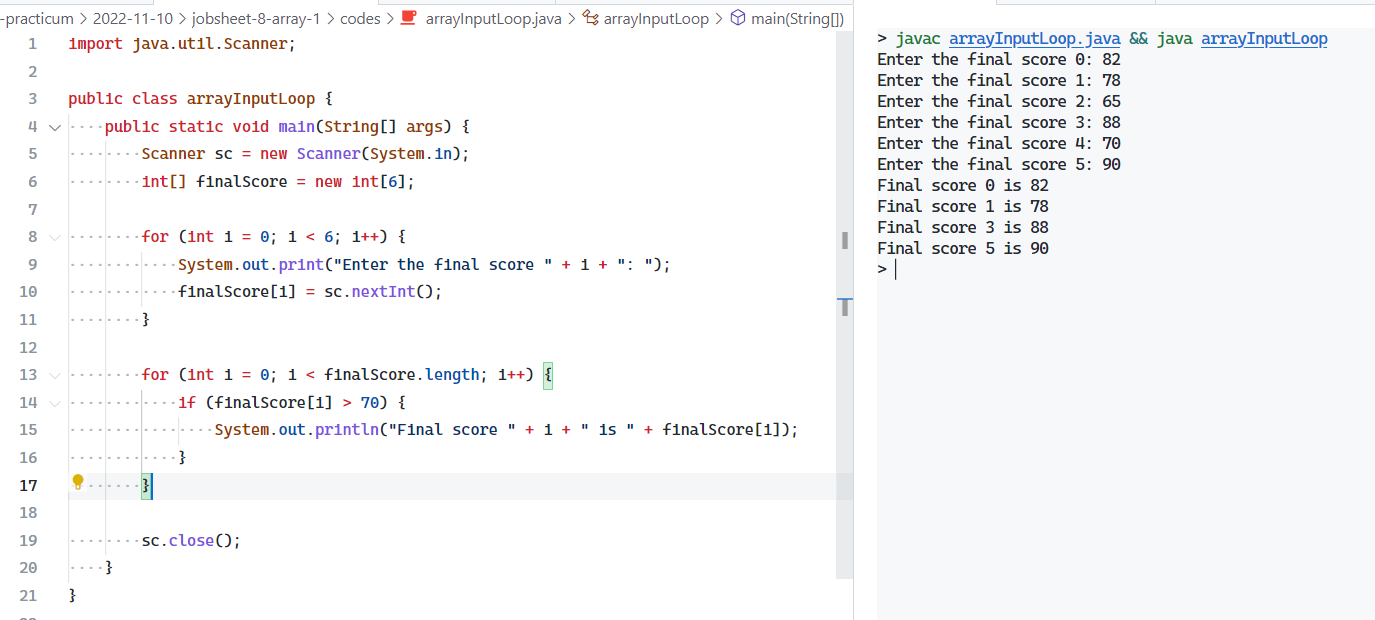
\includegraphics[width=.9\textwidth]{./images/arrayInputLoop-if.png}}
            \caption{Experiment 2 with $>$70 scores}
        \end{figure}
    }
    \item {
        Modify the program so that it displays all students, and marked which one passed and which did not!

        \begin{minted}[autogobble]{bash}
            Enter the final score 0: 82
            Enter the final score 1: 78
            Enter the final score 2: 65
            Enter the final score 3: 88
            Enter the final score 4: 70
            Enter the final score 5: 90
            Student 0 Passed
            Student 1 Passed
            Student 2 Failed
            Student 3 Passed
            Student 4 Failed
            Student 5 Passed
        \end{minted}

        \begin{figure}[h]
            \centering
            \fbox{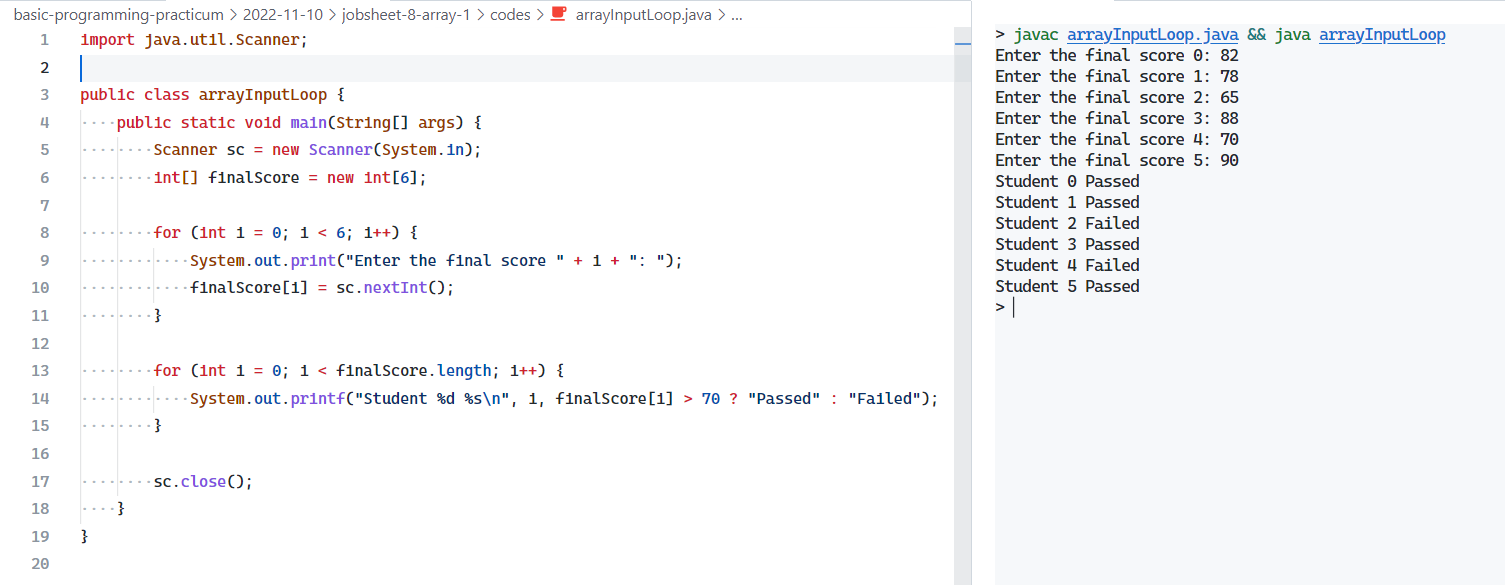
\includegraphics[width=.9\textwidth]{./images/arrayInputLoop-passed.png}}
            \caption{Experiment 2 with Passed or Failed text}
        \end{figure}
    }
\end{enumerate}
\subsection{Experiment 3: Perform Arithmetic Operations on Array Elements}
\begin{enumerate}
    \item {
        This experiment is done to add array elements. The program will accept input of 10 student scores.
        Then the program wil display the average score of 10 students.
    }
    \item Create a new class, name it \texttt{averageScore}
    \item Write the basic structure of the Java programming language which contains the \texttt{main()} function
    \item Add the Scanner library
    \item Make a \textbf{Scanner} declaration with the name \texttt{sc}
    \item {
        Create an array of integer type with the name \texttt{score} with a capacity of 10.
        Then declare the variables total and average

        \begin{minted}[autogobble]{java}
            int[] score = new int[10];
            double total = 0;
            double average;
        \end{minted}
    }
    \item {
        Using a loop, create an input to fill in the \texttt{score} array element
        
        \begin{minted}[autogobble]{java}
            for (int i = 0; i < score.length; i++) {
                System.out.print("enter student score " + (i + 1) + ": ");
                score[i] = sc.nextInt();
            }
        \end{minted}
    }
    \item {
        Using a loop, calculate the total number of scores.

        \begin{minted}[autogobble]{java}
            for (int i = 0; i < score.length; i++) {
                total += score[i];
            }
        \end{minted}
    }
    \item {
        Calculate the average value by dividing \texttt{total} by the number of elements of \texttt{score}

        \begin{minted}[autogobble]{java}
            average = total / score.length;
            System.out.println("The class average score is " + average);
        \end{minted}
    }
    \pagebreak
    \item {
        Compile and run the program. Match the results of the running programs that you have created according to the following display

        \begin{minted}[autogobble]{bash}
            Enter student score 1: 98
            Enter student score 2: 73
            Enter student score 3: 86
            Enter student score 4: 82
            Enter student score 5: 95
            Enter student score 6: 68
            Enter student score 7: 90
            Enter student score 8: 71
            Enter student score 9: 78
            Enter student score 10: 84
            The class average score is 82.5
        \end{minted}

        \begin{figure}[h]
            \centering
            \fbox{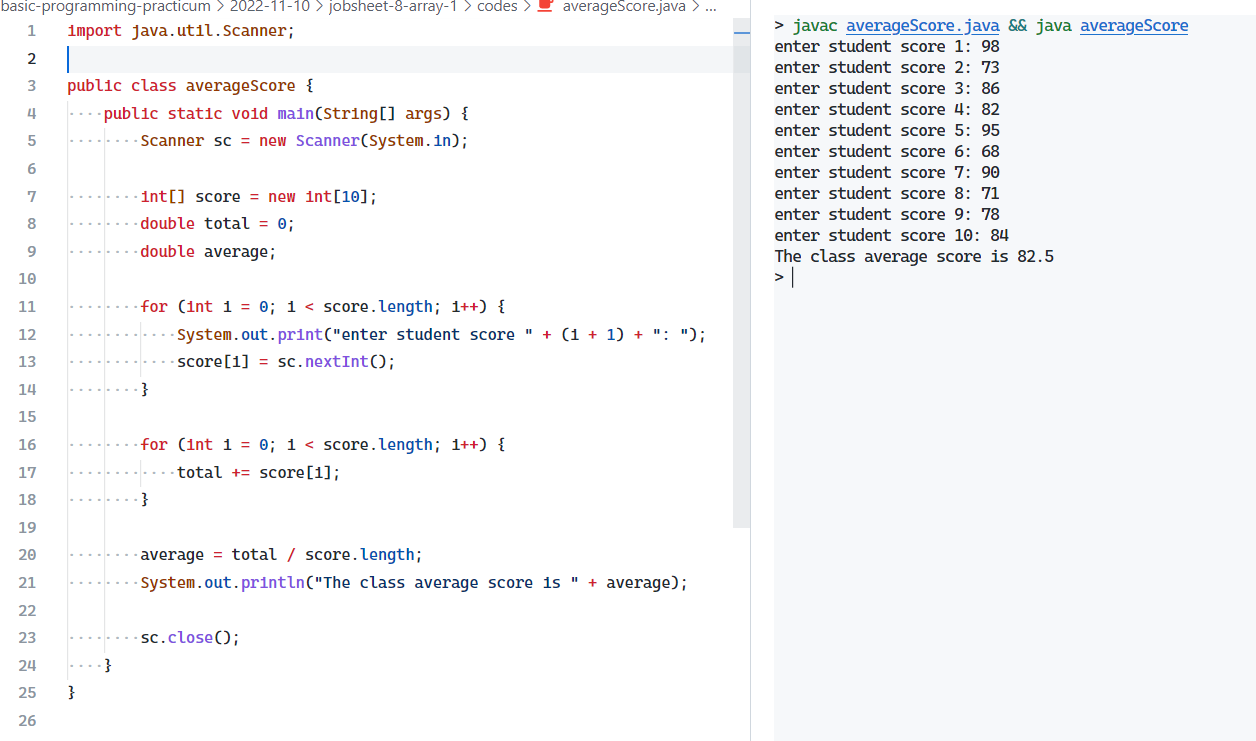
\includegraphics[width=.9\textwidth]{./images/averageScore.png}}
            \caption{Experiment 3 code and output}
        \end{figure}
    }
\end{enumerate}
\subsubsection*{Questions!}
\begin{enumerate}
    \item {
        In step 9, why is the average calculation written outside the loop?

        Because we want to calculate the average once and we need to wait for all of the scores to be accumulated into the \texttt{total} variable.
    }
    \pagebreak
    \item {
        Modify the program in Experiment 3 so that i can produce output like the following display

        \begin{minted}[autogobble]{bash}
            Enter the number of students: 6
            Enter student score 1: 75
            Enter student score 2: 68
            Enter student score 3: 83
            Enter student score 4: 92
            Enter student score 5: 88
            Enter student score 6: 70
            The class average score is 79.3333333333
        \end{minted}

        \begin{figure}[h]
            \centering
            \fbox{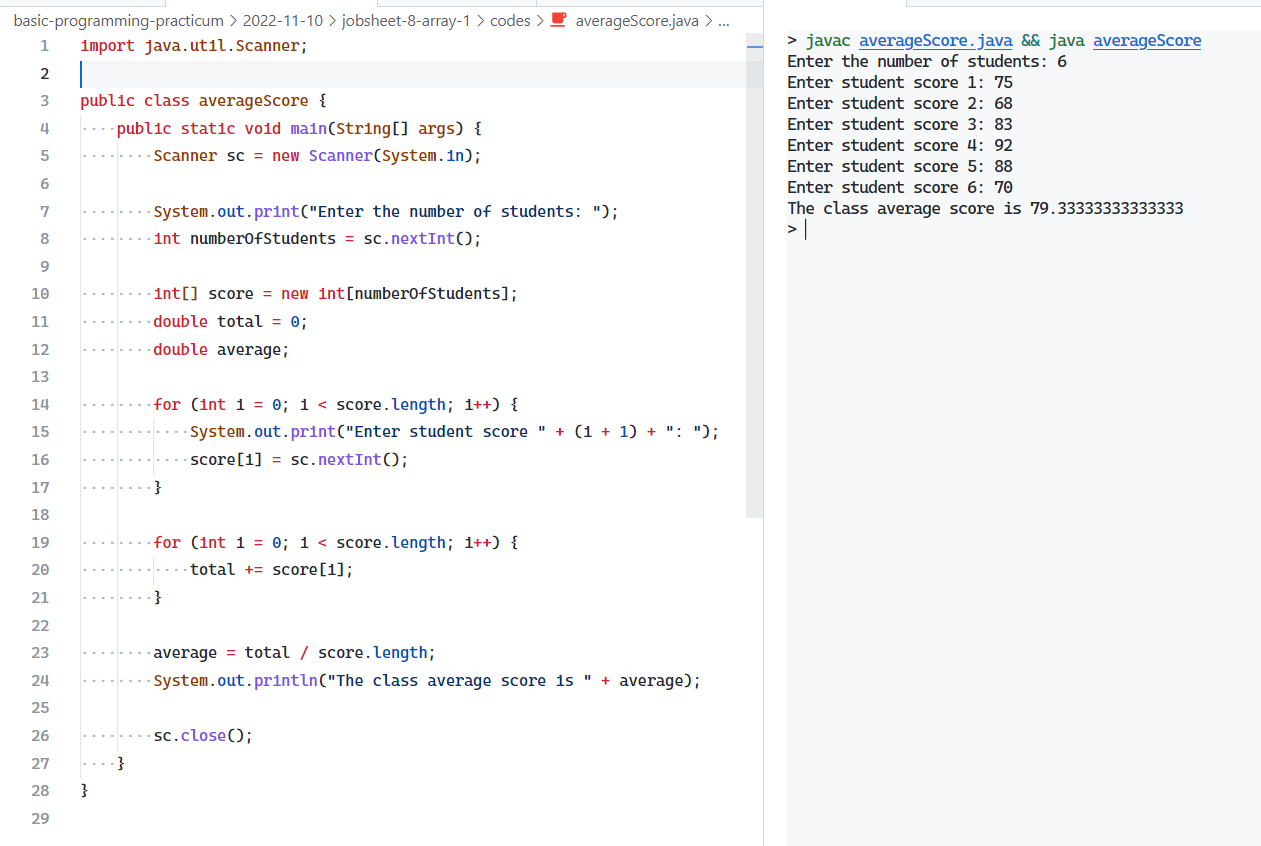
\includegraphics[width=.9\textwidth]{./images/averageScore-input.png}}
            \caption{Experiment 3 with number of students input}
        \end{figure}
    }
\end{enumerate}

\pagebreak

\section{Assignment}
\begin{enumerate}
    \item {
        Create a program that has an array of 5 elements. Then use the input to fill in
        the array elements, and display the contents of the array in reverse order as in the following illustration (figure \ref{array-illustration}).

        \begin{figure}[h]
            \centering
            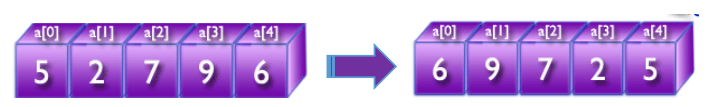
\includegraphics[width=.8\textwidth]{./images/array-illustration.png}
            \caption{Array Illustration}
            \label{array-illustration}
        \end{figure}

        \begin{figure}[h]
            \centering
            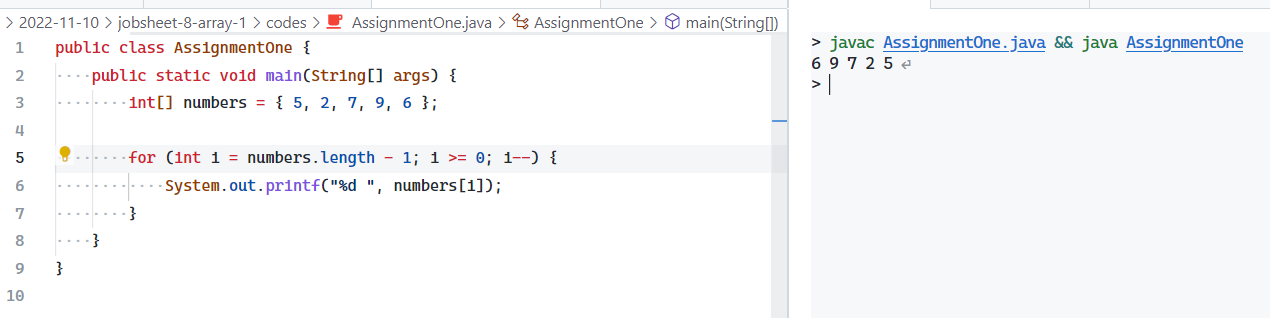
\includegraphics[width=.8\textwidth]{./images/assignment-one.png}
            \caption{Assignment 1 code and output}
        \end{figure}
    }
    \pagebreak
    \item {
        Create a program that accepts the number of array elements as input, also input the elements of array.
        Then display the largest number of the array elements. Examples of program results are as follows:

        \begin{minted}[autogobble]{bash}
            Enter the number of array elements: 4
            Enter the value of element 1: 27
            Enter the value of element 2: 8
            Enter the value of element 3: 33
            Enter the value of element 4: 11
            The largest number is 33
        \end{minted}

        \begin{figure}[h]
            \centering
            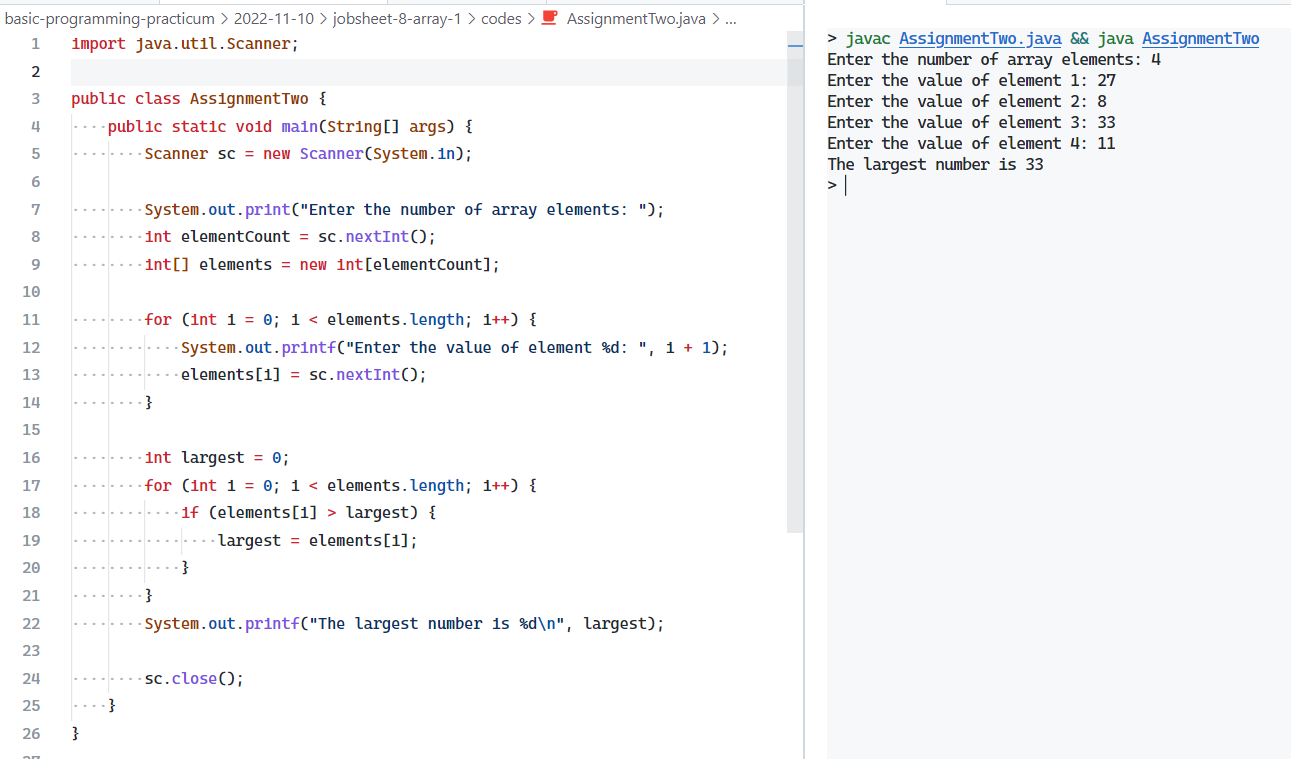
\includegraphics[width=.8\textwidth]{./images/assignment-two.png}
            \caption{Assignment 2 code and output}
        \end{figure}
    }
    \pagebreak
    \item {
        Create a program that accepts the number of array elements as input, also input the elements of array.
        Then display which numbers are even and which are odd numbers. Examples of program results are as follows:

        \begin{minted}[autogobble]{bash}
            Enter the number of array elements: 6
            Enter the value of element 1: 7
            Enter the value of element 2: 3
            Enter the value of element 3: 5
            Enter the value of element 4: 8
            Enter the value of element 5: 2
            Enter the value of element 6: 1
            Even number: 8
            Even number: 2
            Odd number: 7
            Odd number: 3
            Odd number: 5
            Odd number: 1
        \end{minted}

        \begin{figure}[h]
            \centering
            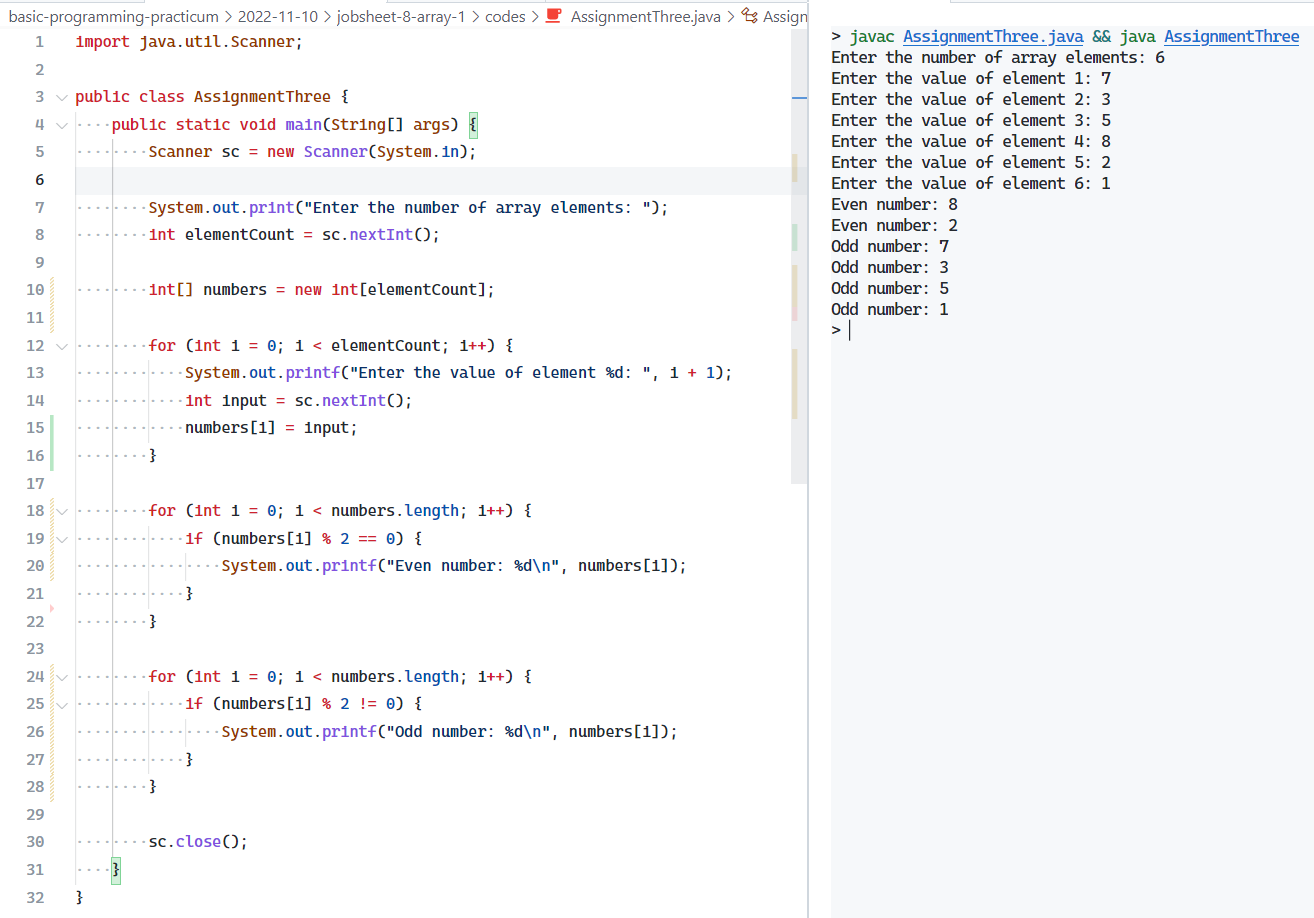
\includegraphics[width=.8\textwidth]{./images/assignment-three.png}
            \caption{Assignment 3 code and output}
        \end{figure}
    }
\end{enumerate}

\end{document}

